

\tikzset{every picture/.style={line width=0.75pt}} %set default line width to 0.75pt        

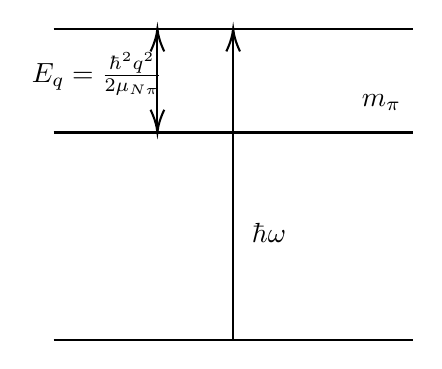
\begin{tikzpicture}[x=0.75pt,y=0.75pt,yscale=-1,xscale=1]
%uncomment if require: \path (0,300); %set diagram left start at 0, and has height of 300

%Straight Lines [id:da9704481650316374] 
\draw    (207,40) -- (380,40) ;
%Straight Lines [id:da8788833386524455] 
\draw    (207,90) -- (380,90) ;
%Straight Lines [id:da2014281021935742] 
\draw    (207,190) -- (380,190) ;
%Straight Lines [id:da43084001692819796] 
\draw    (293.5,190) -- (293.5,42) ;
\draw [shift={(293.5,40)}, rotate = 90] [color={rgb, 255:red, 0; green, 0; blue, 0 }  ][line width=0.75]    (10.93,-3.29) .. controls (6.95,-1.4) and (3.31,-0.3) .. (0,0) .. controls (3.31,0.3) and (6.95,1.4) .. (10.93,3.29)   ;
%Straight Lines [id:da5896583131173334] 
\draw    (257,88) -- (257,42) ;
\draw [shift={(257,40)}, rotate = 90] [color={rgb, 255:red, 0; green, 0; blue, 0 }  ][line width=0.75]    (10.93,-3.29) .. controls (6.95,-1.4) and (3.31,-0.3) .. (0,0) .. controls (3.31,0.3) and (6.95,1.4) .. (10.93,3.29)   ;
\draw [shift={(257,90)}, rotate = 270] [color={rgb, 255:red, 0; green, 0; blue, 0 }  ][line width=0.75]    (10.93,-3.29) .. controls (6.95,-1.4) and (3.31,-0.3) .. (0,0) .. controls (3.31,0.3) and (6.95,1.4) .. (10.93,3.29)   ;

% Text Node
\draw (301,132.4) node [anchor=north west][inner sep=0.75pt]    {$\hbar \omega $};
% Text Node
\draw (354,70.4) node [anchor=north west][inner sep=0.75pt]    {$m_{\pi }$};

% Text Node
\draw (195,50) node [anchor=north west][inner sep=0.75pt]    {$E_q = \frac{\hbar^2 q^2}{2\mu_{N\pi}}$};


\end{tikzpicture}